\documentclass[border=4pt]{standalone}
\usepackage{tikz}
\usetikzlibrary{positioning, arrows.meta, shapes.geometric, calc, fit, backgrounds}
\usepackage{amsmath,amssymb}
\begin{document}
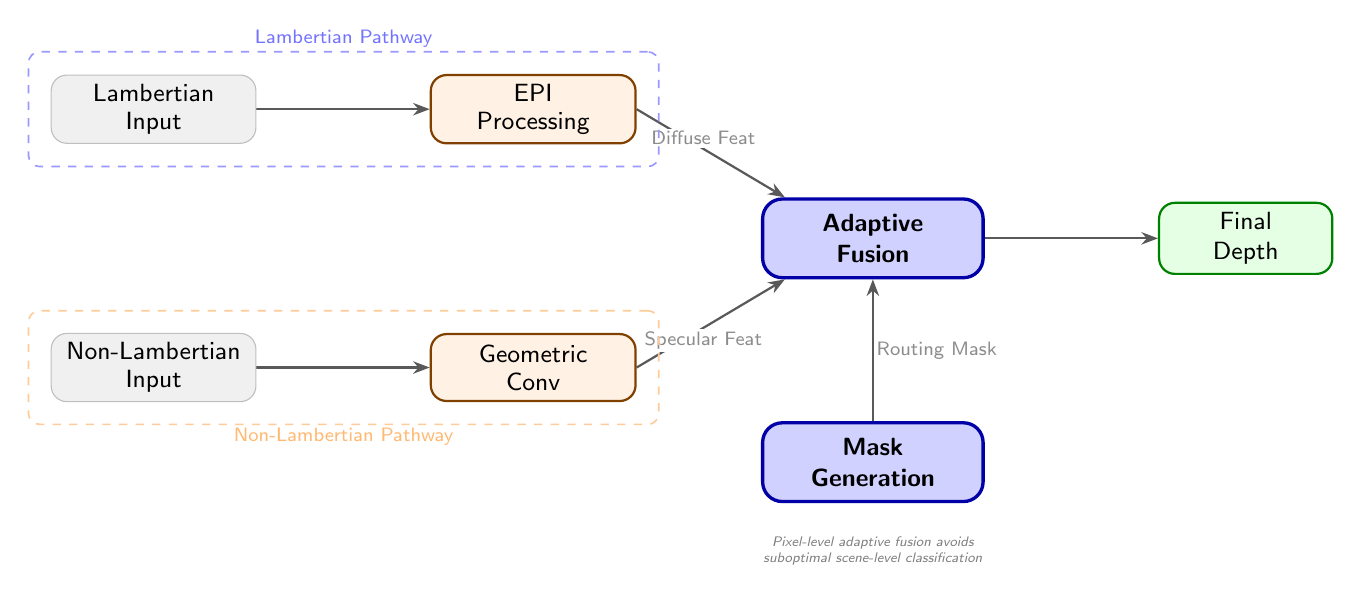
\begin{tikzpicture}[
  input/.style={draw, rounded corners=2mm, minimum width=2.6cm, minimum height=0.85cm,
                fill=gray!12, draw=gray!50, align=center, font=\sffamily\small},
  module/.style={draw, rounded corners=2mm, minimum width=2.6cm, minimum height=0.85cm,
                 fill=orange!10, draw=orange!50!black, line width=0.8pt, align=center,
                 font=\sffamily\small},
  innov/.style={draw, rounded corners=2.5mm, minimum width=2.8cm, minimum height=1.0cm,
                fill=blue!18, draw=blue!65!black, line width=1.2pt, align=center,
                font=\sffamily\small\bfseries},
  output/.style={draw, rounded corners=2mm, minimum width=2.2cm, minimum height=0.85cm,
                 fill=green!10, draw=green!50!black, line width=0.8pt, align=center,
                 font=\sffamily\small},
  arr/.style={-{Stealth[length=6pt]}, thick, color=black!65},
  gbox/.style={draw=#1, dashed, rounded corners=4pt, inner sep=8pt, line width=0.6pt},
  lbl/.style={font=\sffamily\scriptsize, text=black!45, fill=white, inner sep=1pt},
  ann/.style={font=\sffamily\tiny\itshape, text=black!50, align=center},
]

% --- Nodes ---

% Inputs
\node[input] (m1) {Lambertian\\[-1pt]Input};
\node[input, below=2.4cm of m1] (m2) {Non-Lambertian\\[-1pt]Input};

% Processing
\node[module, right=2.2cm of m1] (m3) {EPI\\[-1pt]Processing};
\node[module, right=2.2cm of m2] (m4) {Geometric\\[-1pt]Conv};

% Fusion (centered between m3 and m4)
\path (m3.east) -- (m4.east) coordinate[midway] (mid34);
\node[innov] (m6) at ([xshift=3.0cm]mid34) {\textbf{Adaptive}\\\textbf{Fusion}};

% Mask generation (below m6)
\node[innov, below=1.8cm of m6] (m5) {\textbf{Mask}\\\textbf{Generation}};

% Output
\node[output, right=2.2cm of m6] (m7) {Final\\Depth};

% --- Arrows ---
\begin{scope}[on background layer]
  \draw[arr] (m1) -- (m3);
  \draw[arr] (m2) -- (m4);
  \draw[arr] (m3.east) -- node[lbl, above, pos=0.45] {Diffuse Feat} (m6.155);
  \draw[arr] (m4.east) -- node[lbl, below, pos=0.45] {Specular Feat} (m6.205);
  \draw[arr] (m5.north) -- node[lbl, right, pos=0.5] {Routing Mask} (m6.south);
  \draw[arr] (m6) -- (m7);
\end{scope}

% --- Group Boxes ---
\begin{scope}[on background layer]
  \node[gbox=blue!40, fit=(m1)(m3),
        label={[lbl, text=blue!55]above:Lambertian Pathway}] {};
  \node[gbox=orange!40, fit=(m2)(m4),
        label={[lbl, text=orange!55]below:Non-Lambertian Pathway}] {};
\end{scope}

% --- Annotation ---
\node[ann, below=0.3cm of m5, text width=4.5cm, align=center]
  {Pixel-level adaptive fusion avoids\\suboptimal scene-level classification};

\end{tikzpicture}
\end{document}